\chapter{Entwicklungsumgebung}
\section{Keil MCB1760 Evaluation Board}
Das Keil MCB1760 Evaluation Board enth�lt einen NXP LPC1768 Mikrocontroller basierend auf einem  100Mhz ARM 32-bit Cortex-M3 Mikroprozessor. Neben den wesentlichen Komponenten und Schnittstellen, welche in \autoref{fig:MCB1760EvalBoard} dargestellt sind, verf�gt das Keil MCB1760 Evaluation Board �ber 512KB Flash und 64KB RAM On-Chip Memory.

\begin{figure}[ht!]
	\centering
	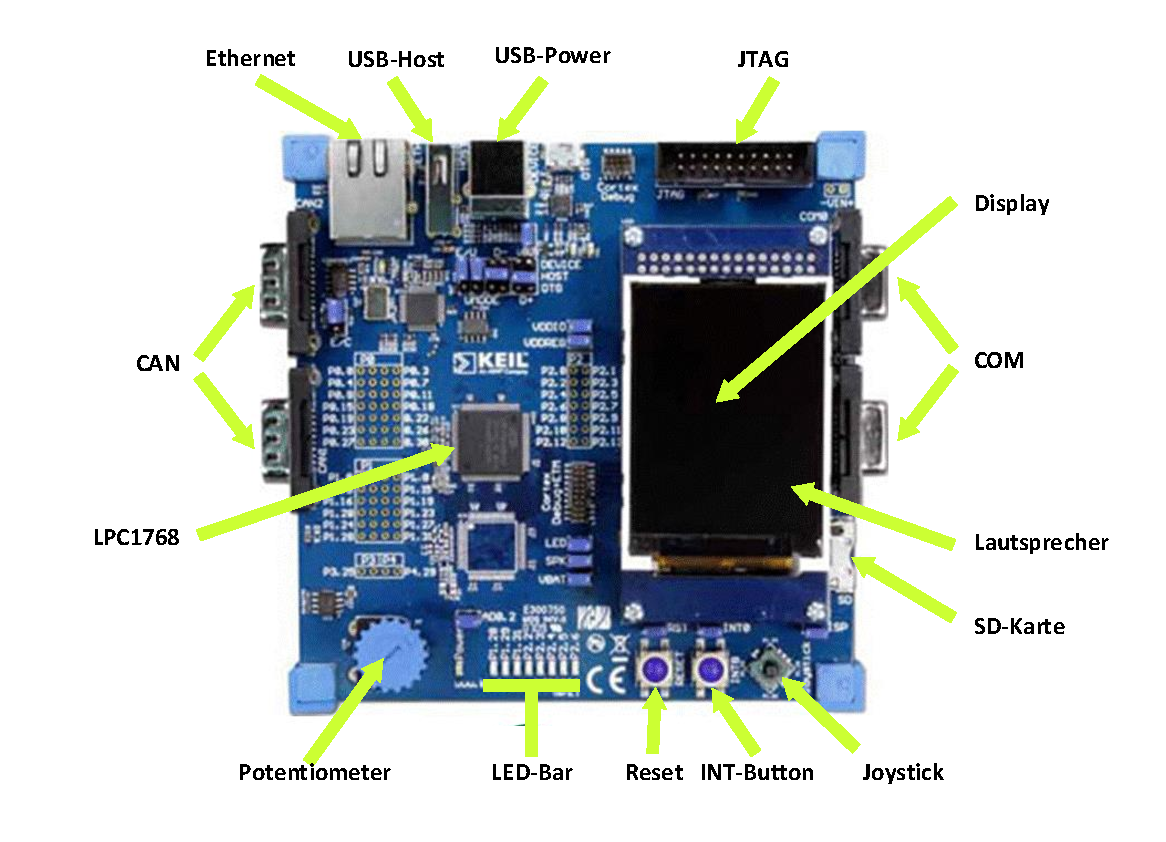
\includegraphics[width=1\textwidth]{images/MCB1700.pdf}
	\caption{Komponenten des MCB1760 Evaluation Board.}
	\label{fig:MCB1760EvalBoard}
\end{figure}

In der Regel werden Evaluation Boards in fr�heren Entwicklungsphasen eingesetzt, um die Leistungsgrenzen der gew�hlten Architektur zu verifizieren. Im Rahmen dieser Arbeit steht die Integration des Evaluation Boards zusammen mit der Toolchain im Vordergrund. 

\section{ESP8266}
TODO
%\begin{figure}[h!]
%	\centering
%		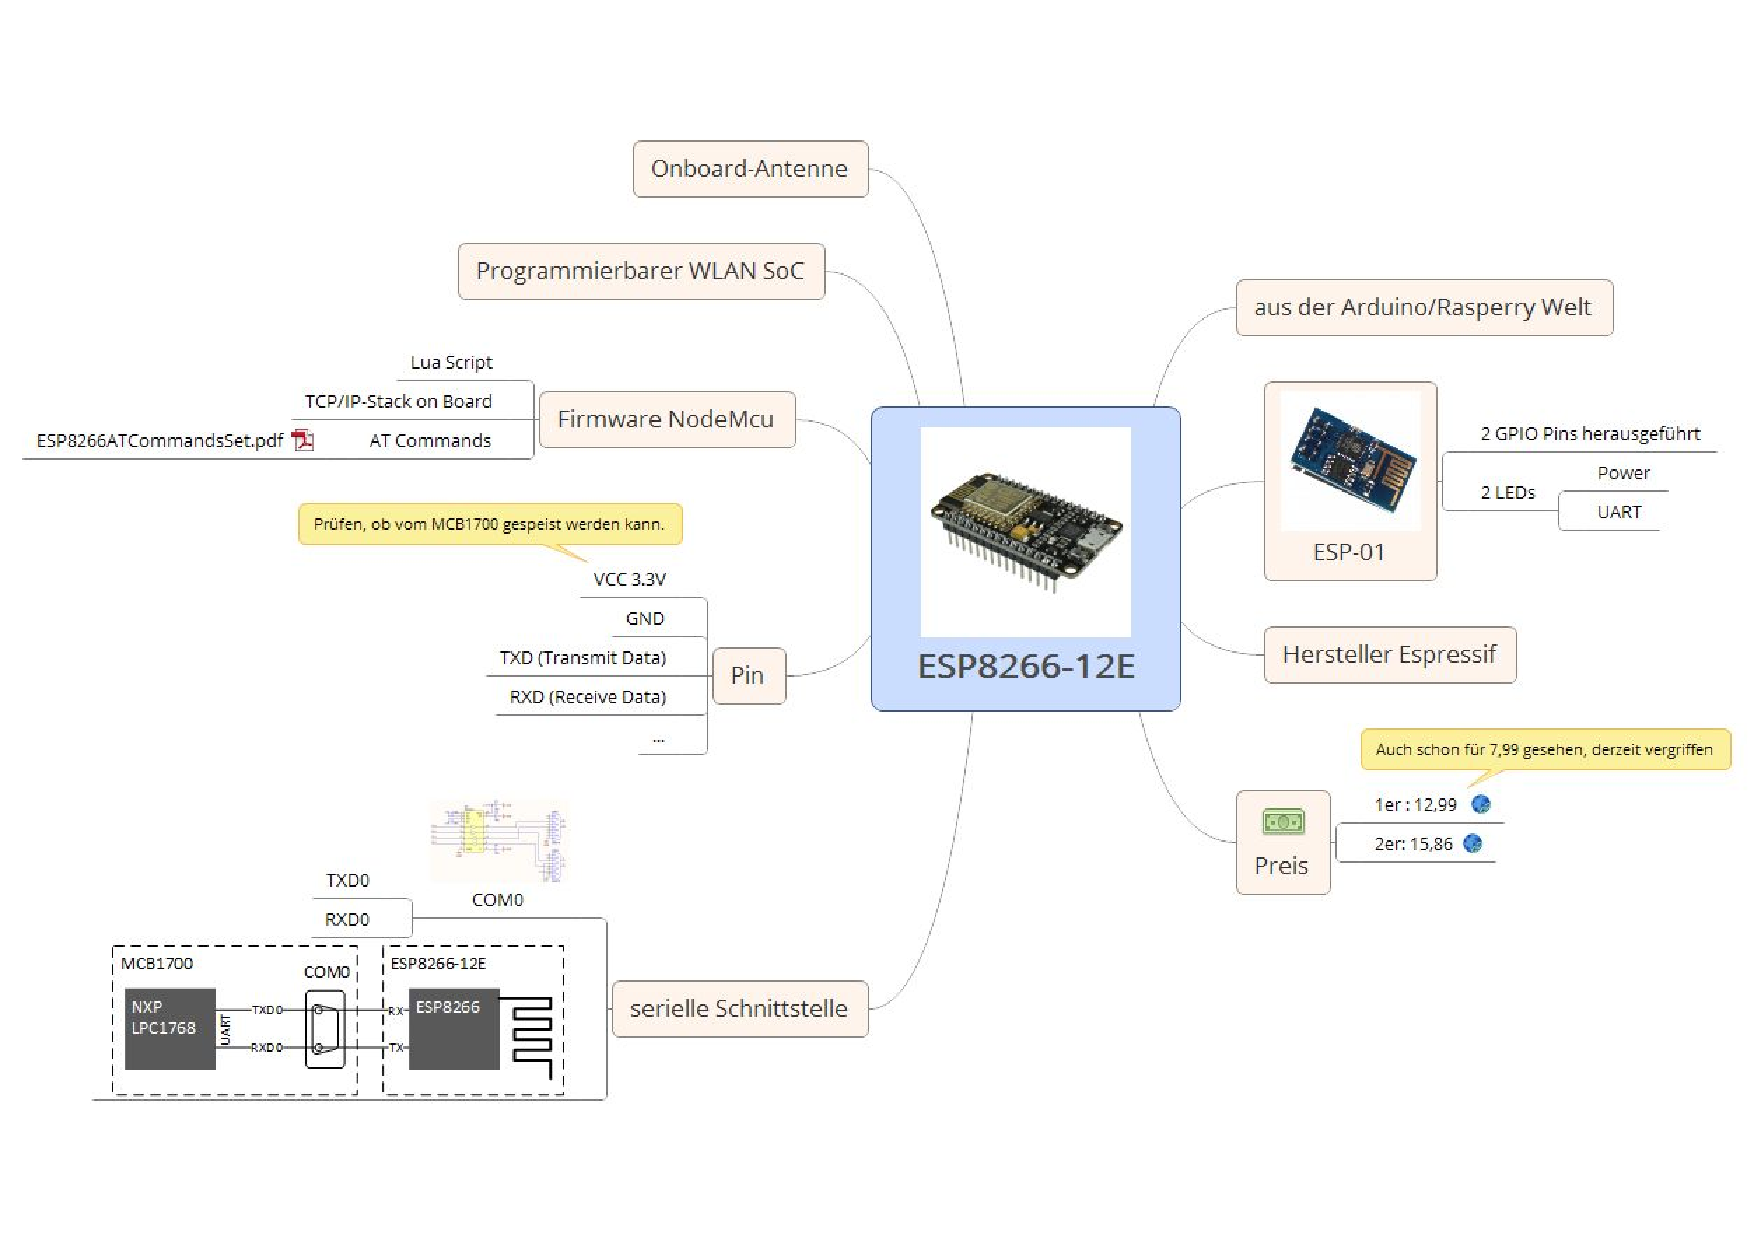
\includegraphics[width=1\textwidth]{images/ESP8266_E12.pdf}
%		\caption[MCB1760 Evaluation Board]{Komponenten des MCB1760 Evaluation Board}
%	\label{schaden}
%\end{figure}

\section{Toolchain}
TODO
\subsection{IBM Rational Rhapsody C++}
TODO
\subsection{Willert Embedded UML RXF}
Der generierte Code aus Rhapsody eignet sich zun�chst nicht zur Ausf�hrung auf einem Target. Die UML-Notation ist viel leistungsst�rker und auf einer h�heren Abstraktionsebene als jede h�here Programmiersprache. UML-Elemente wie asynchrone Kommunikation, aktive Klassen oder auch komplexe Zust�nde k�nnen nicht direkt in eine h�here Programmiersprache �bersetzt werden. 

Das Tool Embedded UML Real-time eXecution Framework (RXF)\abk{$RXF$}{Real-time eXecution Framework} der Firma Willert bildet die Schnittstelle zwischen UML-Modell und einer Zielplattform bestehend aus Compiler, CPU\abk{$CPU$}{Central Processing Unit} und einem m�glichen RTOS\abk{$RTOS$}{Real Time Operating System}. Durch eine Abstraktionsschicht werden die g�ngigsten Echtzeit-Betriebssysteme auf dem Markt unterst�tzt. Das bedeutet, dass in UML definierte Timer oder Events unabh�ngig vom Betriebssystem verwendet werden k�nnen. Somit ist das Software-Design komplett losgel�st vom gew�hlten Target.

Bei der Codegenerierung unterst�tzt das RXF die beiden bekanntesten UML-Tools, Rhapsody und Sparx Enterprise Architect, sowie eine Vielzahl an IDEs\abk{$IDE$}{Integrated Development Environment}. Um eine bestm�gliche Integration zu gew�hrleisten, ist jede Variante des RXF auf die verwendete Toolchain zugeschnitten. Ein Vorteil davon ist, dass die Target IDE �ber das RXF mit Rhapsody verbunden ist und somit der Code aus dem UML-Modell direkt in die Target IDE generiert wird \parencite{ModelingEmSys}. Zur Unterscheidung der vielen verschiedenen Varianten hat die Firma Willert mit der Version 6 einen Produktcode eingef�hrt, welcher zur Identifikation der enthaltenen Komponenten dient. Das Schema ist in der nachfolgenden Tabelle abgebildet.

\begin{table}[ht!]
	\begin{threeparttable}
	\begin{tabular}{cccccc}
		%\hline
			| UML-Tool | Programmiersprache | RTOS | Compiler | EvalBoard\tnote{*} | Zusatz\tnote{**}\hspace{1ex} |\\
		%\hline
		\end{tabular}
		\begin{tablenotes}
			\footnotesize 
			\item[*]{Die EvalBoard Komponente ist kein Teil des Produkts. Sie sagt lediglich aus, mit welcher CPU Familie das Produkt verwendet werden kann.}
			\item[**]{Erweiterungen sind optional und k�nnen auch miteinander kombiniert werden. M�gliche Zus�tze sind "`TD"' f�r Embedded UML Target Debugger oder "`Eval"' f�r eine RXF Evaluierungsversion.}
		\end{tablenotes}
	\end{threeparttable}
	\caption{Produktcode zur Identifikation der enthalten Komponenten \parencite{RXFMigrationGuide}.}
	\label{tab:WillertProduktcode}
\end{table}

In dieser Arbeit wurden die Varianten \begin{itshape}RXF-Eval\_Rpy-Cpp-ARM\end{itshape} in der Version 6.02 und \begin{itshape}Rpy\_CPP\_CMSIS\_Keil5\_ARM\_MCB1700\_TD\end{itshape} in der Version 6.01 verwendet.

\subsection{Keil uVision}
Die IDE Keil uVision ist Teil des Keil Microcontroller Development Kit (MDK)\abk{$MDK$}{Microcontroller Development Kit}. Es vereint einen Projektmanager und eine Run-Time Environment (RTE)\abk{$RTE$}{Run-Time-Environment}, mit deren Hilfe vorgefertigte Software Pakete integriert werden k�nnen. Die Software Pakete k�nnen Bibliotheken, Module, Konfigurationsdateien, Templates und Dokumentation enthalten, welche bei der Inbetriebnahme des Targets unterst�tzen. Die Basisfunktionalit�ten einer gew�hnlichen IDE, wie Quellcode-Editor und Debugger, sind ebenfalls enthalten \parencite{MDK}.

%\begin{figure}[h!]
%	\centering
%		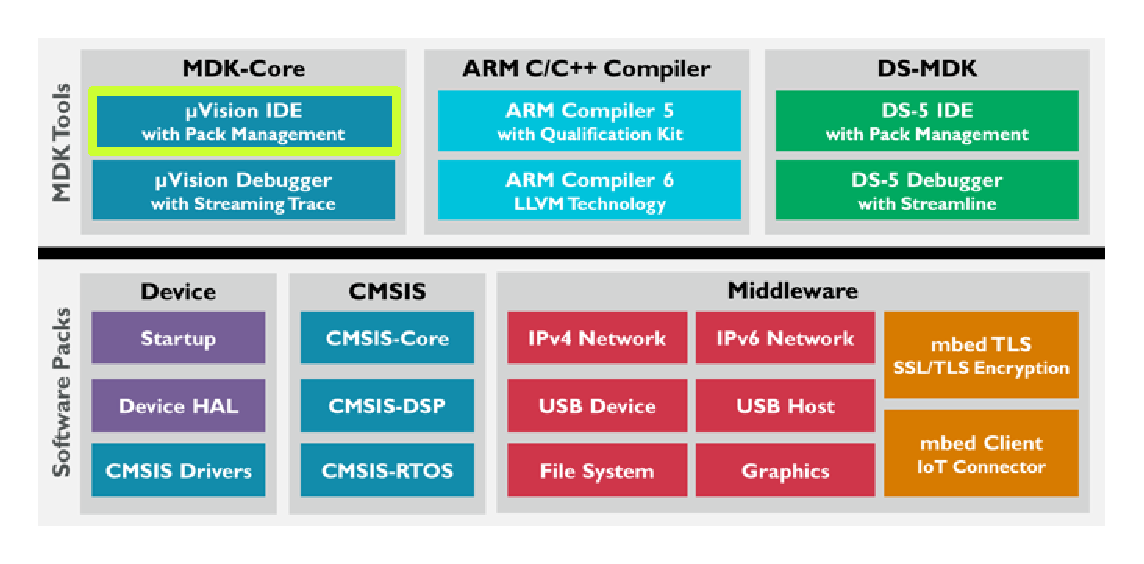
\includegraphics[width=1\textwidth]{images/MDK.pdf}
%		\caption[Keil MDK]{�berblick Keil MDK Version 5}
%	\label{KeilMDK}
%\end{figure}
 
In dieser Arbeit wird das Keil MDK in der Version 5 verwendet. Im Vergleich zum vorherigen Keil MDK in der Version 4, ist eine wesentliche Neuerung das Echtzeitbetriebssystem Cortex Microcontroller Software Interface Standard (CMSIS)\abk{$CMSIS$}{Cortex Microcontroller Software Interface Standard}. Es l�st das bisherige RTX Real-Time Library (RL-ARM)\abk{$RL-ARM$}{Real-Time Library for ARM microprocessors} Echtzeitbetriebssystems ab und bringt die folgenden Vorteile mit sich \parencite{RLARMtoCMSIS}: 

\begin{itemize}
\item Standardisierte API
\item Basisfunktionen zur Unterst�tzung von UML oder Java
\item Einfaches wiederverwenden von Software Komponenten durch einheitliche Funktionen
\item CMSIS konforme Middleware kann einfach angepasst werden
\end{itemize}
